% DOCUMENT CLASS
\documentclass[letterpaper, 10 pt, conference]{ieeeconf}
\IEEEoverridecommandlockouts{}
\overrideIEEEmargins{}  % required to meet printer requirements.

% DOCUMENT STRUCTURE
\usepackage{subfiles}

% TABLES
\usepackage{caption}
\usepackage{multirow}

% ALGORITHMS
\usepackage{algorithmic}
\usepackage{algorithm}

% GRAPHICS
\usepackage{float}
\usepackage{subcaption}
\usepackage{tikz}
\usepackage{tikzscale}
%\usepackage{tkzgraph}
\usetikzlibrary{matrix}
\usepackage{verbatim}
\usetikzlibrary{arrows,shapes}
\usetikzlibrary{calc}
\usepackage{graphicx}
\usepackage{hyperref}

% MATH SYMBOLS
\usepackage{amsfonts} % mathbb{R}
\usepackage{amsmath}
\DeclareMathOperator*{\argmin}{arg\,min}

% COMMENT BLOCKS
\usepackage{verbatim}

% SUBSCRIPT COMMANDS
\newcommand{\superscript}[1]{\ensuremath{^{\textrm{#1}}}}
\newcommand{\subscript}[1]{\ensuremath{_\textrm{#1}}}

% TITLE
\title{\large \textbf Autonomous Quadrotor Landing on a Moving Platform in
Outdoor Environments}

% AUTHORS
\author{\
Chris Choi\authorrefmark{1}, Stanley Brown\authorrefmark{2} and  Steven L. Waslander\authorrefmark{3}
\thanks{\superscript{*} M.A.Sc. Candidate, Mechanical and Mechatronics Engineering, University of Waterloo; c33choi@uwaterloo.ca}
\thanks{\superscript{2} M.A.Sc. Candidate, Mechanical and Mechatronics Engineering, University of Waterloo; s52brown@uwaterloo.ca}
\thanks{\superscript{\dag} Assistant Professor, Mechanical and Mechatronics Engineering, University of Waterloo; stevenw@uwaterloo.ca}
\vspace{0.5in}
}

\begin{document}
\maketitle
\thispagestyle{empty}
\pagestyle{empty}

% ABSTRACT
\begin{abstract}
\end{abstract}


% INTRODUCTION
\section{Introduction}

% RELATED WORK
\section{Related Work}


% CONTRIBUTION
\section{Contribution}

\begin{itemize}
  \item{Robust Landing}
  \item{AprilTag estimation with Kalman Filter}
  \item{AprilTag windowing to speed up detection}
  \item{Light Invariant AprilTag detection}
  \item{Tracking Controller}
  \item{Trajectory Planning}
\end{itemize}

% SYSTEM OVERVIEW
\section{System Overview}
In this section we describe the setup of our problem, from the quadrotor,
ground landing target to coordinate systems used to represent positions in
body and inertial frames.

For the autonomous landing problem we assume that the quadrotor has direct line
of sight to the landing target and that the AprilTag is detectable. The target
position and velocity estimation is performed on-board the quadrotor, and
using the estimations of the target the quadrotor tracks and lands onto the
target.

\begin{itemize}
  \item{$I$\@: Inertial Frame}
  \item{$C$\@: Camera Frame}
  \item{$G$\@: Gimbal Frame}
  \item{$B$\@: Quadrotor Body Frame}
  \item{$BP$\@: Quadrotor Body Planar Frame}
\end{itemize}

We describe five different main coordinate frames used throughout this
paper, in general we have followed the ROS coordinate frame conventions
where the inertial frame $I$ is in ENU coordinate frame, the camera frame
$C$ is in EDN coordinate frame, gimbal frame $G$, quadrotor body frame $B$ and
quadrotor body planar frame $BP$ uses NWU coordinate frame. The quadrotor body
planar frame $BP$ is defined as the body centered and inertial horizon $x$-$y$
aligned frame, to reiterate the body planar frame $BP$ ignores the roll and
pitch (but not yaw) normally considered in a body frame $B$.



% TARGET TRACKING
\section{Target Tracking}
A popular visual fiducial system called AprilTag~\cite{Olson2011} was chosen,
the system allows us to identify the landing target along with the full 6 dof
estimation. There exists multiple implementations of
AprilTag,~\cite{AprilTagMIT} was chosen because it is the most used
implementation. In the following we describe steps taken to optimize the
AprilTag detection in-order to run the processing at a higher rate.


\subsection{Adaptive Image Processing}
The standard implementation of the AprilTag library when processing images
of 640 by 480 pixels results with an update rate of approximately 3 to
5 fps on the on-board computer too low for quadrotor controls. To improve
performance we adapted the image size depending on the estimated
distance between camera and AprilTag.

\subsection{AprilTag Windowing}
In~\cite{Ling2014} an attempt was made to optimize the AprilTag library
by reducing the brightness of the image such that the majority of the
image is black, we went one step further and masked the lastest image
using the last detected AprilTag camera coordinates, rendering everything
other than the AprilTag black, with this modification we assumed the image
coordinates between frames did not vary too wildly, else the mask is
removed and the full image is inputed to the AprilTag detector for
processing.

Once the center of the AprilTag in camera frame is found the top left and
bottom right corners of the AprilTag can be calculated with:

\begin{align}
  X_{\text{top left}} &= X - (l / 2) - X_{\text{padding}} \\
  Y_{\text{top left}} &= Y - (l / 2) - Y_{\text{padding}} \\
  X_{\text{bottom right}} &= X + (l / 2) + X_{\text{padding}} \\
  Y_{\text{bottom right}} &= Y + (l / 2) + Y_{\text{padding}}
\end{align}

Where $X, Y$ are positions of the AprilTag in the camera frame,
$X_{\text{padding}}, Y_{\text{padding}}$ are the mask padding in the camera
frame, $l$ is the AprilTag side length in meters, and finally $X_{\text{top
left}}, Y_{\text{top left}}, X_{\text{bottom right}}, Y_{\text{bottom right}}$
represent the top left and bottom right corners in the camera frame. Adding the
mask padding at this point allows the padding to be defined in the camera
frame which increases and decreases proportionally in the image frame
depending on the depth-distance between camera and AprilTag.

Using the pin-hole camera model, we can convert the AprilTag's corners
from camera frame into image frame with the following:

\begin{equation}
  x = \dfrac{f_{x} * X}{Z}
\end{equation}

\begin{equation}
  y = \dfrac{f_{y} * Y}{Z}
\end{equation}

Where $f_{x}$ and $f_{y}$ are the focal length in pixels in the $x$ and
$y$ axis, and finally $x, y$ are image pixel coordinates. Using the
image coordinates of the top left and bottom right corners of the AprilTag
a mask can be created.

\subsection{Nested AprilTag}
To address visibility issues of the AprilTag as the field of view of is reduced
during landing, we found a unique combination of AprilTag ids that allows us to
place a smaller AprilTag in the center of a larger AprilTag (see
Fig~\ref{fig:apriltag_illumination_invariant}). By shear coincidence the
AprilTag implementation~\cite{AprilTagMIT} always prefers the smaller secondary
tag when both are detected.

\subsection{Illumination Invariant AprilTag}
A common issue in computer vision is illumination changes in the
environment which in turn interferes with the performance of detection
algorithms. From our experience the standard black and white AprilTag
fails to be detected if a shadow is casted partially or fully upon the tag
features, this is because the AprilTag detection relies heavily on the
edges and lines of the tag to be able to estimate the 6 dof pose.
Depending on the time of day or weather conditions, this can have
a significant impact as the quadrotor approaches the target, as its own
shadow over the AprilTag can render the tag undetectable.

Reliable image processing is therefore paramount to the success of target
detection, using methods described in~\cite{Maddern14} we have idenitified
the best colours for an illumination invariant AprilTag to be blue and
green (see Fig~\ref{apriltag_illumination_invariant}), additionally

\begin{equation}
  I = \log(R_{2}) - \alpha \log(R_{1}) - (1 - \alpha) \log(R_{3})
\end{equation}

Where $R_{1}, R_{2}, R_{3}$ are sensor responses (or image channels)
corresponding to peak sensitivies at ordered wavelengths $\lambda_{1}
< \lambda_{2} < \lambda_{3}$.


\begin{figure}
\label{fig:apriltag_illumination_invariant}
  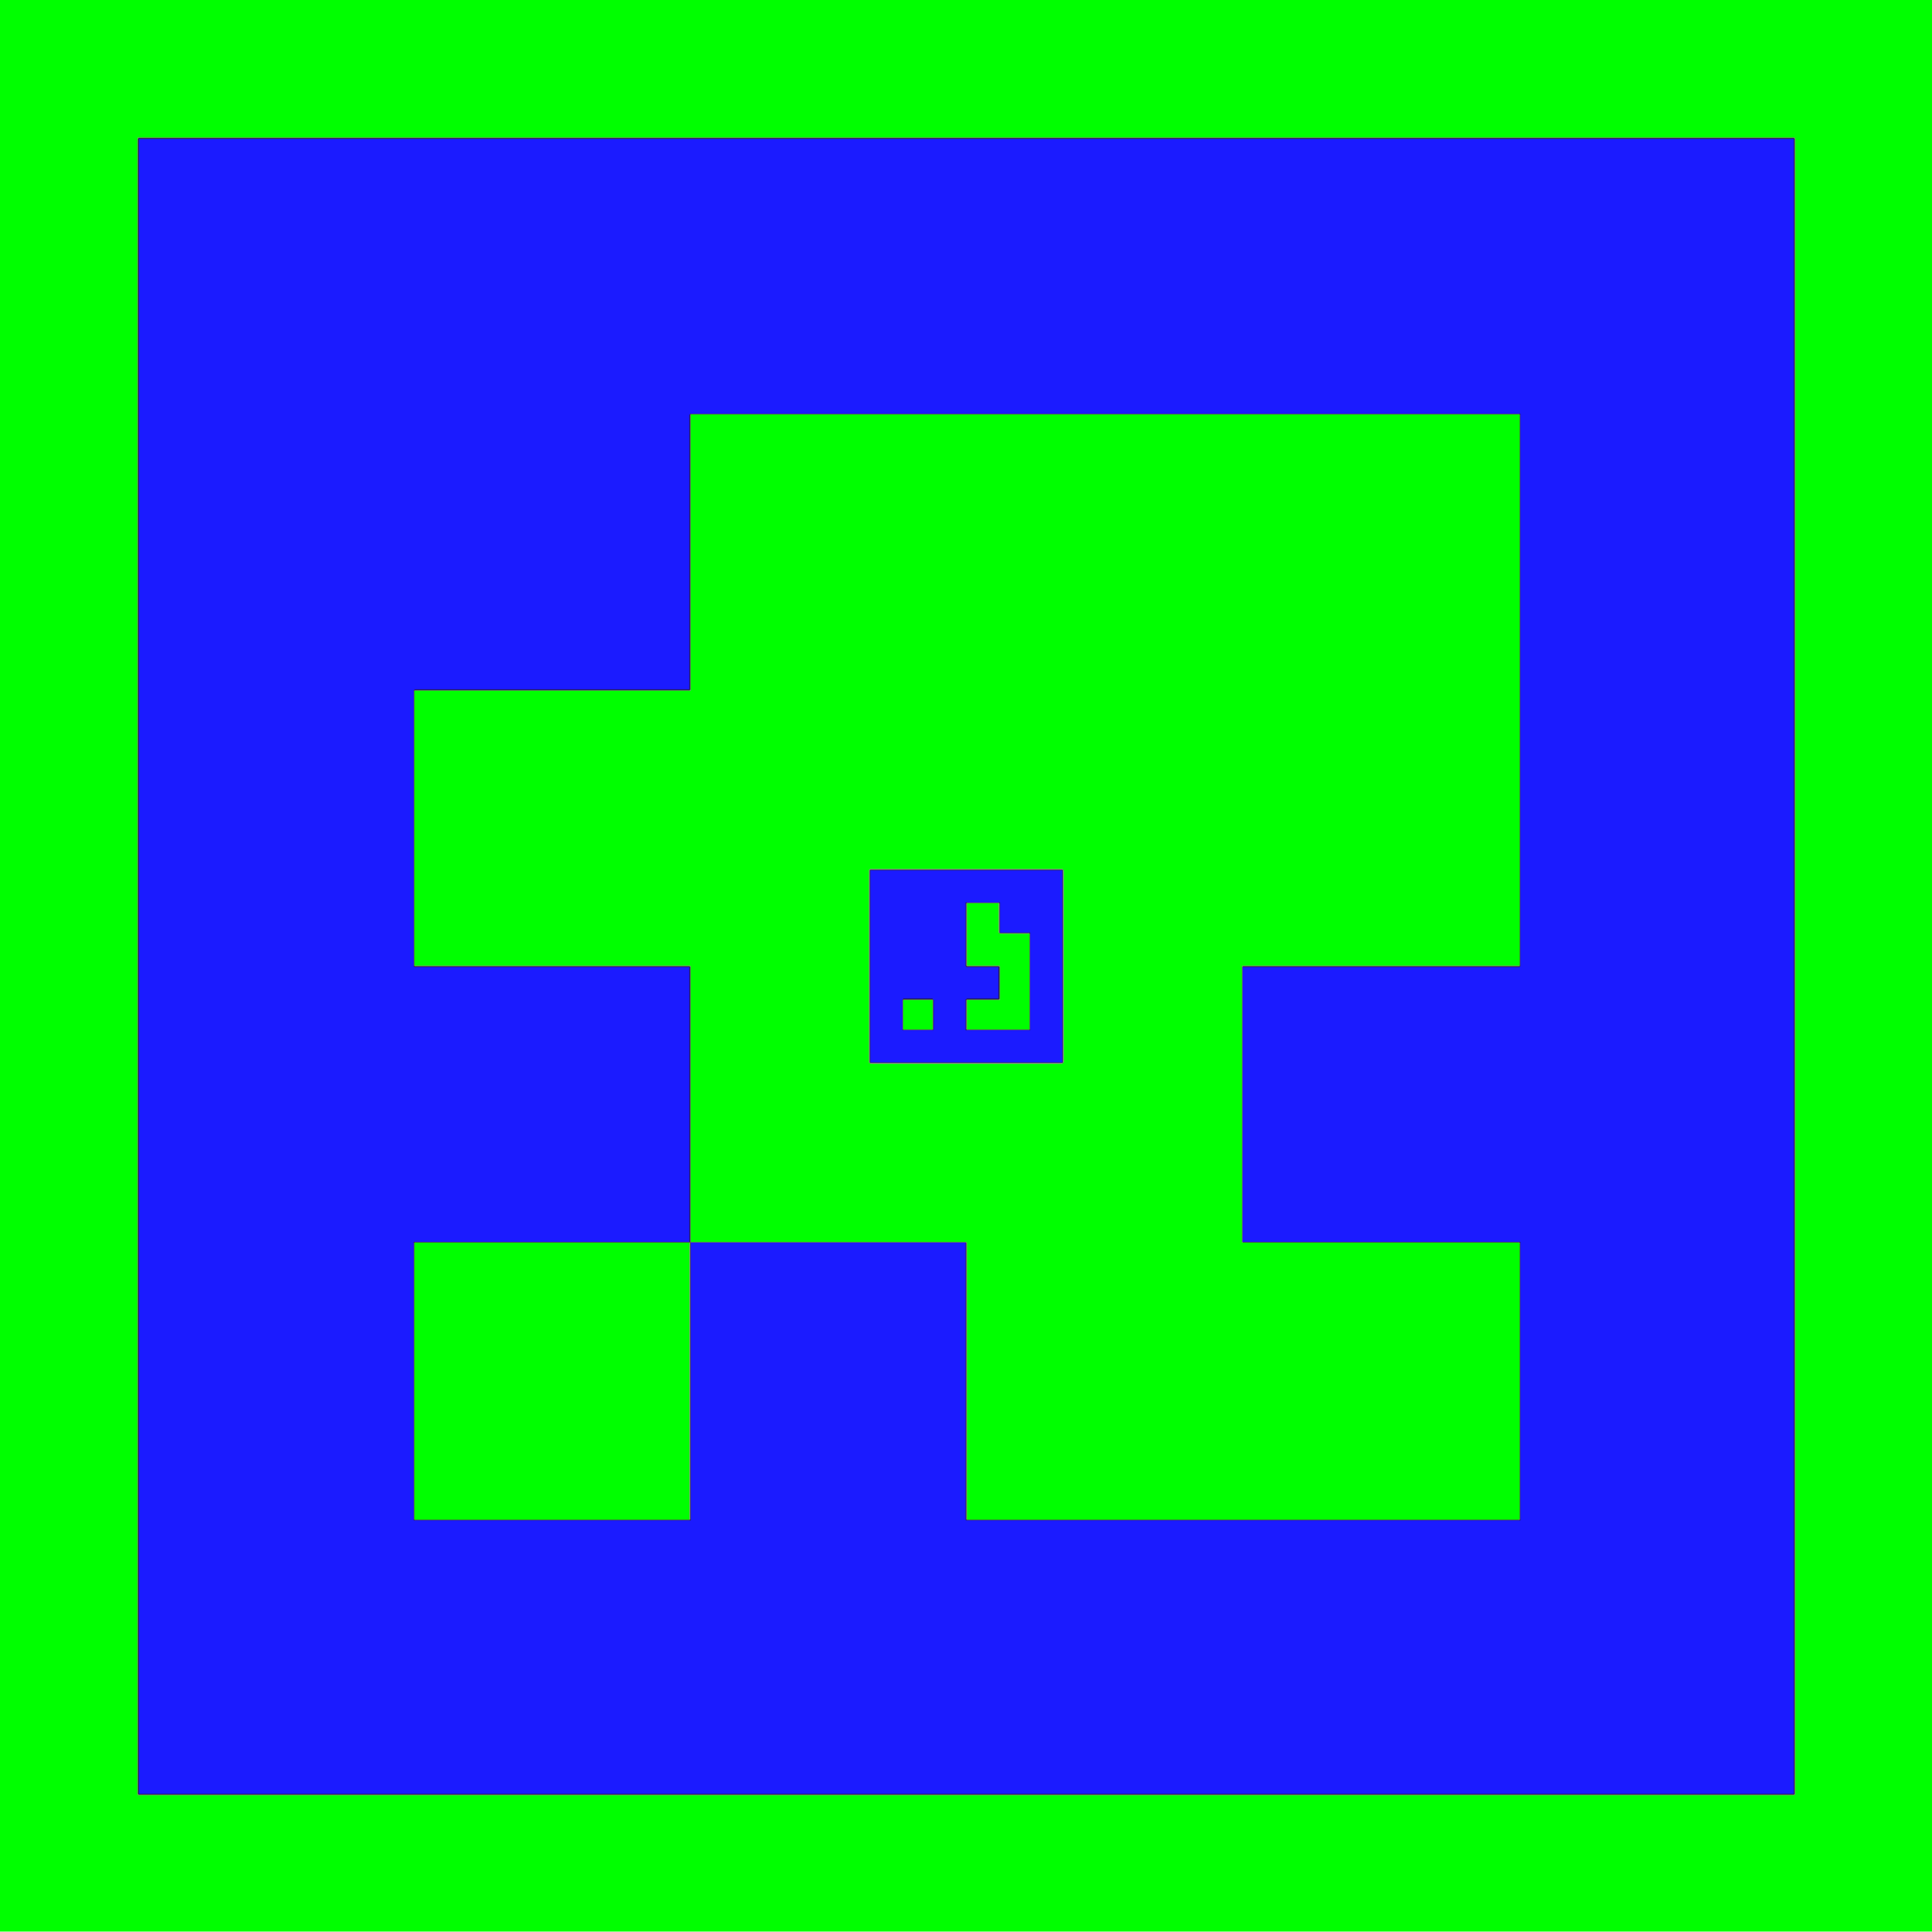
\includegraphics[width=\linewidth]{images/apriltag_illumination_invariant}
  \caption{Illumination Invariant AprilTag}
\end{figure}


% TARGET ESTIMATION
\section{Target Estimation}
The inertial target position, linear velocity, angular velocity and
heading are estimated with an Extended Kalman Filter running at 200Hz, the
estimation is in turn used for tracking and landing controllers on board
the quadrotor.

\subsection{Process Model}
We chose to use a two-wheel robot motion model to approximate the forward
kinematics of the target, which is given as:

\begin{equation}
    \begin{split}
        \textbf{x}
        &= \begin{bmatrix}
            x_{1} & x_{2} & x_{3} & x_{4} & x_{5} & x_{6} & x_{7}
        \end{bmatrix} \\
        &=
        \begin{bmatrix}
            x & y & z & \theta & v & \omega & v_{z}
        \end{bmatrix}
    \end{split}
\end{equation}

\begin{equation}
    \textbf{u}(t)
        = \begin{bmatrix}
            u_{1} \\
            u_{2} \\
            u_{3}
        \end{bmatrix}
        = \begin{bmatrix}
            v \\
            \omega \\
            v_{z}
        \end{bmatrix}
        = \begin{bmatrix}
            \mathcal{N}_{v} \\
            \mathcal{N}_{\omega} \\
            \mathcal{N}_{v_{z}}
        \end{bmatrix}
\end{equation}

\begin{equation}
    \dot{\textbf{x}} = \begin{bmatrix}
        \dot{x_{1}} \\ 
        \dot{x_{2}} \\ 
        \dot{x_{3}} \\ 
        \dot{x_{4}} \\
        \dot{x_{5}} \\
        \dot{x_{6}} \\
        \dot{x_{7}}
    \end{bmatrix} =
    \begin{bmatrix}
        x_{5} \cos(x_{4}) \\
        x_{5} \sin(x_{4}) \\
        x_{7} \\
        x_{6} \\
        u_{1} \\
        u_{2} \\
        u_{3} \\
    \end{bmatrix}
\end{equation}

Where the estimator estimates the inertial position in $x$, $y$ and $z$
direction, heading $\theta$, wheel velocity $v$, steering angular velocity
$\omega$ and linear velocity $v_{z}$ in the $z$ direction. It is worth
noting the linear velocity in the $x$ and $y$ direction can be calculated
from $v \cos(\theta)$ and $v \sin(\theta)$ respectively. The inputs to the
process model are driven by Gaussian White Noise, since we do not possess
input information to the two wheel robot motion model.

\subsection{Measurement Model}
The measurement inputted into the estimator is the target position ($x, y,
z$) in the inertial frame, the target position has been transformed from
the camera frame through to the gimbal frame to the inertial frame. Care
was taken to ensure that the IMU measurements were synchronized with image
of the AprilTag at the time it was captured.

To obtain the target position in the inertial frame, the detected target
position is first transformed from image frame to gimbal joint frame as
follows:

\begin{equation}
  x_{\text{gjf}} = R^{\text{gjf}}_{\text{i}}
    R^{\text{nwu}}_{\text{cf}}
    x_{\text{i}} + t_{c}
\end{equation}

Then from gimbal joint frame to body planar frame:

\begin{equation}
  x_{\text{bpf}} = R^{\text{bpf}}_{\text{gjf}} x_{\text{gjf}}
\end{equation}

Finally from body planar frame to inertial frame:

\begin{equation}
  x_{\text{if}} = R^{\text{enu}}_{\text{nwu}}
    R^{\text{if}}_{\text{bpf}}
    x_{\text{bpf}}
\end{equation}

This final target position in the inertial frame is then passed onto the
estimator. The measurement model $h(t)$ and the linearized measurement
model $H(t)$ at time $t$ is then simply

\begin{equation}
    h(t) = \begin{bmatrix} x, y, z \end{bmatrix}^{T}
\end{equation}

\begin{equation}
    H(t) = \begin{bmatrix} I_{3 \times 3} \end{bmatrix}^{T}
\end{equation}

The Extended Kalman Filter updates the process model at 200 Hz, while the
measurement is updated upon when the AprilTag is detected and transformed.
The output of the estimator is in turn used for tracking and landing.


% TRAJECTORY PLANNING
\section{Trajectory Planning}

\subsection{2D Quadrotor Model}
The model used for trajectory planning is a two dimensional three degrees
of freedom (DOF) quadrotor in the $x$-$z$ plane. By using this model we
assume there will be small changes in the $x$-$y$ plane where the
controllers can correct without planning.

The 2D quadrotor state $\textbf{x}$ includes both position and velocity in the
$x$ and $z$ direction. Where $x_{0}$ and $x_{d}$ are the initial and final
states of the quadrotor. The inputs to the quadrotor model are the
acceleration $a_{z}$ in the $z$ direction in body frame, and pitch angle
$\theta$ in inertial frame.

\begin{equation}
  \begin{split}
    \textbf{x}
      &= \begin{bmatrix}
        x_{1} & x_{2} & x_{3} & x_{4}
      \end{bmatrix}^{T} \\ 
      &= \begin{bmatrix}
        x & \dot{x} & z & \dot{z}
      \end{bmatrix}^{T} \in {\rm I\!R}^{4}
  \end{split}
\end{equation}

\begin{equation}
  \begin{split}
    \textbf{x}_{0} = \begin{bmatrix}
        x_{0} & \dot{x_{0}} & z_{0} & \dot{z_{0}}
    \end{bmatrix}^{T} \\
    \textbf{x}_{d} = \begin{bmatrix}
        x_{d} & \dot{x_{d}} & z_{d} & \dot{z_{d}}
    \end{bmatrix}^{T}
  \end{split}
\end{equation}

\begin{equation}
  \textbf{u}(t)
    = \begin{bmatrix} u_{1} \\ u_{2} \end{bmatrix}
    = \begin{bmatrix} a_{z} \\ \theta \end{bmatrix}
    \in {\rm I\!R}^{2}
\end{equation}

The dynamics are thus given as:

\begin{equation}
  \dot{\textbf{x}} =
    \begin{bmatrix}
      \dot{x_{1}} \\ \dot{x_{2}} \\ \dot{x_{3}} \\ \dot{x_{4}}
    \end{bmatrix} =
    f(\textbf{x}, \textbf{u}) =
    \begin{bmatrix}
      x_{2} \\
      u_{1} \sin(u_{2}) \\
      x_{4} \\
      u_{1} \cos(u_{2}) - g \\
      u_{2}
    \end{bmatrix}
\end{equation}

Where $g$ is the gravitational constant.

\subsection{Trajectory Problem Formulation}
The objective of the trajectory is to achieve landing of the quadrotor
onto a non-stationary target at $\textbf{x}_{d}$, further the trajectory
has to satisfy a number of desirable soft constraints, which are minimal
deviation from desired path $p_{\text{diff}}$, minimal total input
$u_{\text{total}}$ and minimal input control difference between time steps
$u_{\text{diff}}$.

The desired path $\textbf{p}_{\text{desired}}$ vector is a straight-line
from initial position $x_{0}$ to final position $x_{d}$. 

\begin{equation}
    p_{\text{diff}} = || \textbf{x} - \textbf{p}_{\text{desired}} ||^{2}
\end{equation}

\begin{equation}
    u_{\text{total}} = || \textbf{u} ||^{2}
\end{equation}

\begin{equation}
    u_{\text{diff}} = \sum_{i = 0}^{t_{f} - 1}
        \left\Vert
            \textbf{u}(i + 1) - \textbf{u}(i)
        \right\Vert^{2}
\end{equation}

\begin{equation}
    J(\textbf{x}, \textbf{u}) =
        w_{1} \cdot p_{\text{diff}}
        + w_{2} \cdot u_{\text{total}}
        + w_{3} \cdot u_{\text{diff}}
\end{equation}

\begin{equation}
  C_{\text{eq}} = \sum_{i = 0}^{t_{f} - 1}
    \textbf{x}(i + 1) - f(\textbf{x}(i), \textbf{u}(i))
\end{equation}

\begin{align}
  \text{minimize} \quad &J(\textbf{x}, \textbf{u}) \\
  \text{s.t.} \quad & \dot{\textbf{x}} = f(\textbf{x}, \textbf{u}) \\
    & \textbf{x}(t = 0) = \textbf{x}_{0} \\
    & \textbf{x}(t = t_{f}) = \textbf{x}_{d} \\
    & \textbf{u} \in \textbf{U} \quad \forall t \in [0, t_{f}]
\end{align}


% QUADROTOR CONTROL
\section{Quadrotor Control}

\subsection{Tracking Controller}
For target tracking two PID controllers were implemented, first a position
based controller that corrects positional errors of the quadrotor relative
to the target. Second, a velocity based controller that uses estimated
target velocity as a feed-forward signal to match the target's velocity.
The two controllers are combined together to form the tracking controller.

\begin{equation}
   \theta = k_{p} e + k_{i} \sum_{i = 0}^{t} e_{i} dt + k_{d} \dot{e}
\end{equation}

\begin{figure}
\label{fig:tracking_controller}
  \includegraphics[width=\linewidth]{images/tracking_controller}
  \caption{Tracking Controller}
\end{figure}

\subsection{Landing Controller}
During landing the controller will be switched from tracking to landing,
the controller contains two PID controllers the first controller is
a position based control to correct positional errors of the quadrotor
relative to the target in the body frame.




% EXPERIMENT RESULTS
\section{Experiment Results}



% CONCLUSIONS
\section{Conclusions and Future Work}

% BIBLIOGRAPHY
\bibliography{paper}
\bibliographystyle{ieeetr}

\end{document}
